\newpage

\section{Class \Iclass{conic}} % (fold)
\label{sec:class_iclass_conic}

\subsection{Preamble} % (fold)
\label{sub:preamble}
To illustrate the different methods used to draw conics, here's how you can obtain a parabola. In the following example, the parabola is the locus of all circle centers tangent to a given circle.

The \code{points} table contains the coordinates of the centers of the identified circles. \TIKZ only requires a list of coordinate pairs enclosed in brackets.
The table that defines the circles is slightly more complex. It contains the centers and the tangency points between the circles and the given elements. These are sequences of four coordinates, stored in the table. Finally, the sequences are concatenated into a string using a comma (",") as the separator. Coordinates are read with the \tkzcname{foreach} macro, utilizing the |expand list| option.

\directlua{
init_elements()
z.O = point : new (0,0)
z.P = point : new (0,6)
z.M = point : new (0,3)
z.I = point : new (1,0)
C.PM = circle : new (z.P,z.M)
list = {}
points = {}
 for t = -0.24, 0.24, 0.004 do
 if (t> - 0.002 and t< 0.002) then else
     z.A   = C.PM : point (t)
     L.OI  = line : new (z.O,z.I)
     L.PA  = line : new (z.P,z.A)
     z.C   = intersection (L.OI,L.PA)
     L.tgt = C.PM : tangent_at (z.A)
     z.X   = intersection (L.tgt,L.OI)
     z.o   = bisector (z.X,z.A,z.C).pb
     table.insert (points, "("..z.o.re..","..z.o.im..")")
     table.insert (list,z.o.re.."/"..z.o.im.."/"..z.A.re.."/"..z.A.im)
   end
   end
  list = table.concat(list,",")
 }

\begin{center}
  \begin{tikzpicture}[scale=0.5]
  \tkzGetNodes
  \tkzDrawCircle(P,M)
     \foreach[expand list] \r/\s/\u/\v in {\directlua{tex.print({list})}}
      {
        \tkzDefPoint(\u,\v){A}
        \tkzDefPoint(\r,\s){o}
        \tkzDrawCircle[orange](o,A)
      }
   \tkzDrawCoordinates[smooth,red](points)
  \end{tikzpicture}
\end{center}

Here's the code. Two lists are created, one containing the points of the parabola, the other the points that define the tangent circles.
The parabola is obtained using \TIKZ{}'s ability to draw a curve from a list of coordinates. To obtain the circles, note the use of the \code{expand list} option in the \tkzcname{foreach} loop.

\begin{Verbatim}
  \directlua{
  z.O = point : new (0,0)
  z.P = point : new (0,6)
  z.M = point : new (0,3)
  z.I = point : new (1,0)
  C.PM = circle : new (z.P,z.M)
  list = {}
  points = {}
   for t = -0.24, 0.24, 0.004 do
   if (t> - 0.002 and t< 0.002) then else
       z.A   = C.PM : point (t)
       L.OI  = line : new (z.O,z.I)
       L.PA  = line : new (z.P,z.A)
       z.C   = intersection (L.OI,L.PA)
       L.tgt = C.PM : tangent_at (z.A)
       z.X   = intersection (L.tgt,L.OI)
       z.o   = bisector (z.X,z.A,z.C).pb
       table.insert (points, "("..z.o.re..","..z.o.im..")")
       table.insert (list,z.o.re.."/"..z.o.im.."/"..z.A.re.."/"..z.A.im)
     end
     end
    list = table.concat(list,",")
   }
\end{Verbatim}

  \begin{Verbatim}
    \begin{tikzpicture}[scale =.75]
    \tkzGetNodes
    \tkzDrawCircle(P,M)
       \foreach[expand list] \r/\s/\u/\v in {\directlua{tex.print({list})}}
        {
          \tkzDefPoint(\u,\v){A}
          \tkzDefPoint(\r,\s){o}
          \tkzDrawCircle[orange](o,A)
        }
     \tkzDrawCoordinates[smooth,red](points)
    \end{tikzpicture}
  \end{Verbatim}





% subsection preamble (end)

This class replaces the one dedicated to ellipses. From now on, you can work with parabolas, hyperbolas and ellipses. The circle is not part of this class.
As you'll see from the examples, ellipses used to be built by \TIKZ{}, now conics are obtained by point-by-point construction. A cloud of points is sent to \TIKZ{}, which simply connects them.

\begin{mybox}
  \begin{Verbatim}
    plot[<local options>]coordinates{<coordinate 1><coordinate 2>…<coordinate n>} 
  \end{Verbatim}
\end{mybox}

is used by the macro \tkzcname{tkzDrawCoordinates}. One advantage of this method is that you can easily draw only part of a conic.

\subsection{Attributes of a conic} % (fold)
\label{sub:attributes_of_a_conic}

Parabolas, hyperbolas and ellipses share many attributes, but some exist only for the last two conics. I previously defined ellipses using three points (center, vertex, and covertex), but from now on, conics will be defined using a focus, a directrix, and an eccentricity. Of course, the old method can still be used. I've created a few little conversion tools to get the focus, the director and the eccentricity right in some cases.

The first attributes are used to define the conic:  :  \Iattr{conic}{Fa} (focus) ,  \Iattr{conic}{directrix} (directrix) and  \Iattr{conic}{e} (eccentricity).



\bgroup
\catcode`_=12
\small
\captionof{table}{Conic attributes.}\label{conic:att}
\begin{tabular}{ll}
\toprule
\textbf{Attributes}   & \textbf{Application}\\
\Iattr{conic}{Fa} & main foyer of the conic\\
\Iattr{conic}{directrix} & directrix of the conic\\
\Iattr{conic}{major\_axis} & Axis through focal points\\
\Iattr{conic}{minor\_axis} & Axis through focal points\\
\Iattr{conic}{e} & eccentricity of the conic\\
\Iattr{conic}{type} & The type is 'conic'\\
\Iattr{conic}{subtype} & 'parabola', 'hyperbola' or 'ellipse'\\
\Iattr{conic}{a} & Only for hyperbola and ellipse\\
\Iattr{conic}{b} & Only for hyperbola and ellipse\\
\Iattr{conic}{c} & Only for hyperbola and ellipse\\
\Iattr{conic}{p} & semi latus rectum\\
\Iattr{conic}{slope} & Slope of the line passes through the foci\\
\Iattr{conic}{K} & Projection of the focus onto the directrix\\
\Iattr{conic}{Fb} & Second focus for hyperbola and ellipse\\
\Iattr{conic}{vertex} & main vertex\\
\Iattr{conic}{covertex} & \\
\Iattr{conic}{Rx} & Radius from center to vertex\\
\Iattr{conic}{Ry} & Radius from center to covertex\\
\bottomrule %
\end{tabular}
\egroup


\subsubsection{About attributes of conic} % (fold)
\label{ssub:about_attributes_of_conic}

The figure below and the associated table show common attributes and differences according to exentricity values.

\begin{minipage}{.5\textwidth}
\begin{Verbatim}
\directlua{
 init_elements()
 z.A = point : new ( 0 , 0 )
 z.B = point : new ( 4 , -2 )
 L.dir = line : new (z.A,z.B)
 z.F = point : new ( 2 , 2)
 CO1 = conic : new(z.F,L.dir,.8)
 CO2 = conic : new(z.F,L.dir, 1)
 CO3 = conic : new(z.F,L.dir, 1.2)
 curve1 = CO1 : points (0,1, 40)
 curve2 = CO2 : points (-5,5,40)
 curve3 = CO3 : points (-5,5,40)
 z.K = CO1.K
 z.u,z.v = get_points(CO1.major_axis)
 z.x = L.dir : report (-4,z.K)
 z.y = L.dir : report ( 4,z.K)
 z.r = (z.F-z.K) : orthogonal (-4) : at (z.F)
 z.s = (z.F-z.K) : orthogonal (4) : at (z.F)
 L.rs = line : new (z.r,z.s)
 z.I_1   = intersection (L.rs,CO1)
 z.I_2 = intersection (L.rs,CO2)
 z.I_3,_ = intersection (L.rs,CO3)
 z.H_1 = CO1.directrix : projection (z.I_1)
 z.H_2 = CO2.directrix : projection (z.I_2)
 z.H_3 = CO3.directrix : projection (z.I_3)
 z.S_2 = CO2.vertex
 z.F_1 = CO1.Fb
 z.C_1 = CO1.center
 z.C_3 = CO3.center
}

\begin{tikzpicture}
\tkzGetNodes
 \tkzDrawLines(x,y u,v r,s)
 \tkzDrawPoints(F,K,I_1,I_2,I_3,S_2,H_1,H_2,H_3,F_1,C_1,C_3)
 \tkzLabelPoints(F,K,H_1,H_2,H_3,F_1,C_1,C_3)
 \tkzDrawSegments[dashed](I_1,H_1 I_2,H_2 I_3,H_3)
 \tkzLabelPoints[above](I_1,I_2,I_3,S_2)
 \tkzDrawCoordinates[smooth](curve1)
 \tkzDrawCoordinates[smooth](curve2)
 \tkzDrawCoordinates[smooth](curve3)
 \tkzLabelSegment[pos=.4](K,F){$h = KF$}
 \tkzLabelSegment[sloped,pos=-.2](x,y){\texttt{directrix}}
\end{tikzpicture}
\end{Verbatim}
\end{minipage}
\begin{minipage}{.5\textwidth}
\directlua{
init_elements()
z.A = point : new ( 0 , 0 )
z.B = point : new ( 4 , -2 )
L.dir = line : new (z.A,z.B)
z.F = point : new ( 2 , 2)
CO1 = conic : new(z.F,L.dir,.8)
CO2 = conic : new(z.F,L.dir, 1)
CO3 = conic : new(z.F,L.dir, 1.2)
curve1 = CO1 : points (0,1, 40)
curve2 = CO2 : points (-5,5,40)
curve3 = CO3 : points (-5,5,40)
z.K = CO1.K
z.u,z.v = get_points(CO1.major_axis)
z.x = L.dir : report (-4,z.K)
z.y = L.dir : report ( 4,z.K)
z.r = (z.F-z.K) : orthogonal (-4) : at (z.F)
z.s = (z.F-z.K) : orthogonal (4) : at (z.F)
L.rs = line : new (z.r,z.s)
z.I_1   = intersection (L.rs,CO1)
z.I_2 = intersection (L.rs,CO2)
z.I_3,_ = intersection (L.rs,CO3)
z.H_1 = CO1.directrix : projection (z.I_1)
z.H_2 = CO2.directrix : projection (z.I_2)
z.H_3 = CO3.directrix : projection (z.I_3)
z.S_2 = CO2.vertex
z.F_1 = CO1.Fb
z.C_1 = CO1.center
z.C_3 = CO3.center
}

\begin{center}
  \begin{tikzpicture}[scale=.6]
  \tkzGetNodes
   \tkzDrawLines(x,y u,v r,s)
   \tkzDrawPoints(F,K,I_1,I_2,I_3,S_2,H_1,H_2,H_3,F_1,C_1,C_3)
   \tkzLabelPoints(F,K,H_1,H_2,H_3,F_1,C_1,C_3)
   \tkzDrawSegments[dashed](I_1,H_1 I_2,H_2 I_3,H_3)
   \tkzLabelPoints[above](I_1,I_2,I_3,S_2)
   \tkzDrawCoordinates[smooth](curve1)
   \tkzDrawCoordinates[smooth](curve2)
   \tkzDrawCoordinates[smooth](curve3)
   \tkzLabelSegment[pos=.4](K,F){$h = KF$}
   \tkzLabelSegment[sloped,pos=-.2](x,y){\texttt{directrix}}
  \tkzText[draw,
  inner sep=10pt,
  line width = 1pt,
  text width=6cm](2,14){The focus $F$, the line \code{directrix} and  the value of $h =KF$ are attributes common to all three conics. These conics differ in their eccentricity $e$, here $0.8$ for the ellipse, $1$ for the parabola and $1.2$ for the hyperbola. The \code{semi latus rectum} $p$ is equal to $e*h$ and differs depending on the conic. It is represented by $FI_1$, $FI_2$ and $FI_3$. By definition, $\displaystyle e = \frac{p}{h}$}
  \end{tikzpicture}
\end{center}
\end{minipage}


\subsubsection{Attributes of  parabola} % (fold)
\label{ssub:attributes_of_parabola}
Let \begin{mybox}
   |PA = conic : new (z.F, L.AB, 1)|
\end{mybox}
The focus is $F$, it is given if we use another definition by \code{PA.Fa}.
The eccentricity of a parabola is always $1$. It has only one focus, unlike the hyperbola and ellipse. The parabola has no center and only one directrix. The parabola can be distinguished from other conics by its eccentricity, of course, but also by \code{subtype}. Thus \code{PA.subtype = 'parabola'}.

The projection of $F$ onto the directrix is the point $K$, which is given by \code{PA.K}.

$p$, the \code{semi latus rectum}, is always given by $e \cdot h$, so here $p = h$.

Like other conics, the parabola has a vertex given by \code{PA.vertex}, but no \code{covertex}. The vertex is the middle of the segment $KF$.

It can be seen that if we choose a reference frame with origin $S$, the parabola has an equation of the style $y = \dfrac{x^2}{2p}$. For conics, the values $a$, $b$, $c$ represent distances from the center, so they don't exist for the parabola.

The last two attributes are common to all conics. They are the axis passing through the focus $F$ and its projected line $K$ on the directrix. This line is obtained with \code{PA.major\_axis}. You can also use the angle between this axis and the horizontal with \code{PA.slope}. The main axis is oriented from $K$ to $F$.
 
\directlua{
 init_elements()
 z.A = point : new ( 0 , 0 )
 z.B = point : new ( 4 , -2 )
 L.dir = line : new (z.A,z.B)
 z.F = point : new ( 2 , 2)
 PA = conic : new(z.F,L.dir, 1)
 curve2 = PA : points (-5,5,20)
 z.K = PA.K
 z.u,z.v = get_points(PA.major_axis)
 z.x = L.dir : report (-4,z.K)
 z.y = L.dir : report ( 4,z.K)
 z.r = (z.F-z.K) : orthogonal (-4) : at (z.F)
 z.s = (z.F-z.K) : orthogonal (4) : at (z.F)
 L.rs = line : new (z.r,z.s)
 _,z.I_2 = intersection (L.rs,PA)
 z.H_2 = PA.directrix : projection (z.I_2)
 z.S_2 = PA.vertex
}

\begin{tikzpicture}
 \tkzGetNodes
 \tkzDrawLines(x,y u,v r,s)
 \tkzDrawPoints(F,K,I_2,S_2,H_2)
 \tkzLabelPoints(F,K,H_2)
 \tkzDrawSegments[dashed](I_2,H_2)
 \tkzLabelPoints[above](I_2,S_2)
 \tkzDrawCoordinates[smooth](curve2)
 \tkzLabelSegment[pos=.4](K,F){$h = p = KF$}
 \tkzLabelSegment[above,pos=.5](F,I_2){$ p = h = FI_2$}
 \tkzLabelSegment[sloped,pos=.8](x,y){\texttt{directrix}}
 \tkzLabelSegment[left](K,S_2){$h/2$}
\end{tikzpicture}
 
% subsubsection attributes_of_parabola (end)

\subsubsection{Attributes of hyperbola} % (fold) attributs de l'hyperbole
\label{ssub:attributes_of_hyperbola}

Let \begin{mybox}
   |HY = conic : new (z.F, L.AB, 1.2)|
\end{mybox}

This time, the eccentricity is greater than $1$. The common attributes have already been mentioned. Specific attributes include second focus (\code{HY.Fb}) and center (\code{HY.center}). 

It's possible to use different measures of the segments that characterize the hyperbola. $CS = a$ the distance between center and vertex is obtained with (\code{HY.a}). $CF = c$ the distance between center and focus is obtained with (\code{HY.c}).


\directlua{
 init_elements()
 z.A     = point : new ( 0 , 0)
 z.B     = point : new ( 4 , -2)
 L.dir   = line  : new (z.A,z.B)
 z.F     = point : new ( 2 , 1.8)
 HY      = conic : new(z.F,L.dir, 2)
 curve   = HY    : points (-6,6,20)
 curves  = HY    : points (-5,5,20,swap)
 z.K     = HY.K
 z.u,z.v = get_points(HY.major_axis)
 z.x     = L.dir : report (-4,z.K)
 z.y     = L.dir : report ( 4,z.K)
 z.r     = (z.F-z.K) : orthogonal (-5) : at (z.F)
 z.s     = (z.F-z.K) : orthogonal ( 5) : at (z.F)
 L.rs    = line : new (z.r,z.s)
 _,z.I   = intersection (L.rs,HY)
 z.H     = HY.directrix : projection (z.I)
 z.S     = HY.vertex
 z.C     = HY.center
 z.G     = HY.Fb
 z.E     = HY.covertex
 z.D     = (z.S-z.C) : orthogonal (HY.b): at (z.S)
}

\begin{center}
\begin{tikzpicture}
  \tkzGetNodes
  \tkzDrawLines(x,y r,s G,F)
  \tkzDrawLine[red,add= 0 and 1](C,D)
  \tkzDrawLines[add = -.2 and -.2](u,v)
  \tkzDrawPoints(E,F,K,I,S,H,C,G,D)
  \tkzLabelPoints[right](E,F,K,H,C,D,G)
  \tkzDrawSegments[dashed](I,H)
  \tkzDrawPolySeg[dashed](C,E,D,S)
  \tkzLabelPoint[right](F){$F$ focus}
  \tkzLabelPoints[above](I,S)
  \tkzDrawCoordinates[smooth](curve)
  \tkzDrawCoordinates[smooth](curves)
  \tkzLabelSegment[pos=.6,right=8 pt](K,F){$h = KF$}
  \tkzLabelSegment[pos=.6,sloped](I,F){$p  = IF = e*h$}
  \tkzLabelSegment[sloped,pos=.8](x,y){\texttt{directrix}}
  \tkzLabelSegment[sloped,pos=.4](C,D){\color{red}\texttt{asymptote}}
  \tkzLabelSegment[pos=1.6](C,D){\color{red}\texttt{slope = $\displaystyle\frac{b}{a}$}}
  \tkzText[
  inner sep=10pt,
  line width = 1pt,
  text width=4cm](-3,-4){
       $CS = a$\\
       $CF = c$\\
       $CE = b$\\
       slope of asymptote = $\displaystyle\frac{b}{a}$\\
       $IF = p = e*h$\\
       $KF = h$
  }
\end{tikzpicture}
\end{center}

% subsubsection attributes_of_hyperbola (end)

\subsubsection{Attributs of ellipse} % (fold)
\label{ssub:attributs_of_ellipse}

We find the same attributes as for the hyperbola. The relationships between the measures change: while for the hyperbola we have $c = \sqrt{a^2+b^2}$, for the ellipse $c = \sqrt{a^2-b^2}$.

\directlua{
 init_elements()
 z.A     = point : new ( 0 , 0)
 z.B     = point : new ( 4 , -2)
 L.dir   = line  : new (z.A,z.B)
 z.F     = point : new ( 2 , 2)
 HY      = conic : new(z.F,L.dir, .75)
 curve   = HY    : points (0,1,50)
 z.K     = HY.K
 z.u,z.v = get_points(HY.major_axis)
 z.x     = L.dir : report (-4,z.K)
 z.y     = L.dir : report ( 4,z.K)
 z.r     = (z.F-z.K) : orthogonal (-5) : at (z.F)
 z.s     = (z.F-z.K) : orthogonal ( 5) : at (z.F)
 L.rs    = line : new (z.r,z.s)
 z.I,z.J = intersection (L.rs,HY)
 z.H     = HY.directrix : projection (z.I)
 z.V     = HY.vertex
 z.C     = HY.center
 z.G     = HY.Fb
 z.E     = HY.covertex
 z.Ep    = z.C : symmetry (z.E)
}

\begin{center}
  \begin{tikzpicture}[scale=.75]
  \tkzGetNodes
  \tkzDrawLines(x,y I,J G,K)
  \tkzDrawLines[add = -.2 and -.2](u,v)
  \tkzDrawPoints(E,F,K,I,V,H,C,G,E')
  \tkzLabelPoints[right](E,F,K,H,C,G,E')
  \tkzDrawSegments[dashed](I,H E,E')
  \tkzLabelPoint[right](F){$F$ focus}
  \tkzLabelPoints[above right](I,V)
  \tkzDrawCoordinates[smooth](curve)
  \tkzLabelSegment[pos=.6,right=8 pt](K,V){$h = KF$}
  \tkzLabelSegment[pos=.5,above right](I,F){$p  = IF = e*h$}
  \tkzLabelSegment[sloped,pos=.8](x,y){\texttt{directrix}}
  \tkzLabelSegment[sloped,pos=.8](E,E'){\texttt{minor\_axis}}
  \tkzText[
  inner sep=10pt,
  line width = 1pt,
  text width=4cm](-3,0){
       $CV = a$\\
       $CF = c$\\
       $CE = b$\\
       $IF = p = e*h$\\
       $KF = h$
  }
  \end{tikzpicture}
\end{center}

% subsubsection attributs_of_ellipse (end)

% subsubsection about_attributes_of_conic (end)

\subsection{Point-by-point conic construction} % (fold)
\label{sub:point_by_point_conic_construction}


% subsection point_by_point_conic_construction (end)


\subsection{Parabola construction} % (fold)
\label{sub:parabola_construction}


The method is based on the following observation: if a point $M$ belongs to the parabola, then the bisector of the segment from the focus to the projection of $H$ from $M$ onto the directrix is also the bisector of the angle $\widehat{HFT}$ and the tangent to the parabola at the point $M$.

This is the method I chose to construct the set of points representing the parabola.
\vspace{6pt}

\begin{minipage}{.5\textwidth}
\begin{Verbatim}
\directlua{
 z.A     = point : new ( 0 ,  1 )
 z.B     = point : new ( 4  ,  3 )
 z.F     = point : new ( 2  ,  6 )
 L.AB    = line  : new (z.A,z.B)
 PA      = conic : new (z.F,L.AB,1)
 z.K     = PA.K
 z.M     = PA : point(-2)
 z.H     = PA.directrix : projection (z.M)
 L.FH    = line : new (z.F,z.H)
 L.med   = L.FH : mediator ()
 L.orth  = PA.directrix : ortho_from (z.H)
 z.T     = intersection (L.AB,L.med)
 curve   = PA : points (-5,5,50)
 z.m = midpoint(z.H,z.F)
} 
\begin{tikzpicture}
 \tkzGetNodes
 \tkzDrawCoordinates[smooth](curve)
 \tkzDrawLines[add = .5 and .5](A,B M,T K,F)
 \tkzDrawSegments(M,H H,F F,M)
 \tkzDrawPoints(F,K,T,M,H)
 \tkzLabelPoints(F,K,T,M,H)
 \tkzMarkAngles[mark=|](H,M,T T,M,F)
 \tkzMarkSegments[mark=|](H,M M,F)
 \tkzMarkSegments[mark=|](H,m m,F)
\end{tikzpicture}
\end{Verbatim}
\end{minipage}
\directlua{
  init_elements()
   z.A     = point : new ( 0 ,  1 )
   z.B     = point : new ( 4  ,  3 )
   z.F     = point : new ( 2  ,  6 )
   L.AB    = line  : new (z.A,z.B)
   PA      = conic : new (z.F,L.AB,1)
   z.K     = PA.K
   z.M     = PA : point(-2)
   z.H     = PA.directrix : projection (z.M)
   L.FH    = line : new (z.F,z.H)
   L.med   = L.FH : mediator ()
   L.orth  = PA.directrix : ortho_from (z.H)
   z.T     = intersection (L.AB,L.med)
   curve   = PA : points (-4,5,50)
   z.m = midpoint(z.H,z.F)
  } 
\begin{minipage}{.5\textwidth}
\begin{center}
  \begin{tikzpicture}[scale=.75]
  \tkzGetNodes
  \tkzDrawCoordinates[smooth](curve)
  \tkzDrawLines[add = .5 and .4](A,B M,T K,F)
  \tkzDrawSegments(M,H H,F F,M)
  \tkzDrawPoints(F,K,T,M,H)
  \tkzLabelPoints(F,K,T,M,H)
  \tkzMarkAngles[mark=|](H,M,T T,M,F)
  \tkzMarkSegments[mark=|](H,M M,F)
  \tkzMarkSegments[mark=|](H,m m,F)
  \end{tikzpicture}
\end{center}
\end{minipage}


\subsection{Hyperbola construction} % (fold)
\label{sub:hyperbola_construction}

\directlua{
  init_elements()
  z.A     = point : new (-2, -1)
  z.B     = point : new ( 4, 0)
  L.AB    = line : new (z.A,z.B)
  z.F     = point : new (0,3)
  HY      = conic : new (z.F,L.AB,2)
  curve   = HY : points (-5,5,50)
  z.K     = HY.K
  z.S     = HY.vertex
  z.O     = HY.center
  z.X     = HY : point(2)
  z.T     = HY.directrix : report (2,HY.K)
  LT      = HY.major_axis : ll_from (z.T)
  z.u,z.v = get_points(LT)
  LC      = HY.minor_axis
  LS      = LC : ll_from (HY.vertex)
  z.D     = intersection_ll_ (LC.pa,LC.pb,HY.Fa,z.T)
  z.E     = intersection_ll_ (LS.pa,LS.pb,HY.Fa,z.T)   
  z.P,z.Q = intersection_lc_ (LT.pa,LT.pb,z.D,z.E)
  z.C = HY.center
} 
  \begin{center}
    \begin{tikzpicture}[scale = 1]
    \tkzGetNodes
    \tkzDrawCoordinates[smooth,cyan](curve)
    \tkzDrawCircle(D,E)
    \tkzDrawLines(F,C F,D)
    \tkzDrawLines[add = 1 and 1](T,P)
    \tkzDrawPoints(C,F,K,S,T,P,D,E)
    \tkzLabelPoints(C,F,K,S,T,D,E)
    \tkzLabelPoint[below,sloped](A){directrix}
    \tkzLabelPoints[above](P)
    \tkzDrawSegments(A,K T,B)
    \tkzDrawSegments[dashed](S,E K,T C,D)
    \end{tikzpicture}
  \end{center}  

  \begin{Verbatim}
  \directlua{
  z.A     = point : new (-2, -1)
  z.B     = point : new ( 4, 0)
  L.AB    = line : new (z.A,z.B)
  z.F     = point : new (0,3)
  HY      = conic : new (z.F,L.AB,2)
  curve   = HY : points (-5,5,50)
  z.K     = HY.K
  z.S     = HY.vertex
  z.O     = HY.center
  z.X     = HY : point(2)
  z.T     = HY.directrix : report (2,HY.K)
  LT      = HY.major_axis : ll_from (z.T)
  z.u,z.v = get_points(LT)
  LC      = HY.minor_axis
  LS      = LC : ll_from (HY.vertex)
  z.D     = intersection_ll_ (LC.pa,LC.pb,HY.Fa,z.T)
  z.E     = intersection_ll_ (LS.pa,LS.pb,HY.Fa,z.T)   
  z.P,z.Q = intersection_lc_ (LT.pa,LT.pb,z.D,z.E)
  z.C = HY.center
  } 
  \begin{tikzpicture}
  \tkzGetNodes
  \tkzDrawCoordinates[smooth,cyan](curve)
  \tkzDrawCircle(D,E)
  \tkzDrawLines(F,C F,D)
  \tkzDrawLines[add = 1 and 1](T,P)
  \tkzDrawPoints(C,F,K,S,T,P,D,E)
  \tkzLabelPoints(C,F,K,S,T,D,E)
  \tkzLabelPoint[below,sloped](A){directrix}
  \tkzLabelPoints[above](P)
  \tkzDrawSegments(A,K T,B)
  \tkzDrawSegments[dashed](S,E K,T C,D)
  \end{tikzpicture}
  \end{Verbatim}


%subsection hyperbola_construction (end)

\subsection{Ellipse construction} % (fold)
\label{sub:ellipse_construction}

The point-by-point construction is obtained by transforming the principal circle through an affinity with the focal axis as its axis, parallel to the directrix, with a ratio of $b/a$. Let $H$ be the projection of the point $Q$ onto the focal axis. With $OA = a$ and $OB = b$, it is then sufficient to draw a parallel to $(AB)$ passing through $Q$, which intersects the focal axis at $T$, yielding $\dfrac{b}{a} = \dfrac{HT}{HQ}$. Now, since $HT = HQ'$, we obtain $ \dfrac{HQ'}{HQ} = \dfrac{b}{a} $.

\begin{minipage}{.5\textwidth}
\begin{Verbatim}
\directlua{
init_elements()
z.Fb    = point: new ( 3 , 0 )
z.Fa    = point: new ( -3 , 2 )
local c = length(z.Fa,z.Fb)/2
local a = 4
local b = math.sqrt(a^2 -c^2) 
local e = c/a
L.focal = line : new (z.Fa,z.Fb)
z.O     = L.focal.mid
z.K     = report_(z.O,z.Fb,a^2/c)
z.Ko    = ortho_from_(z.K,z.K,z.Fb)
L.dir   = line :new(z.K,z.Ko)
EL      = conic : new (z.Fb,L.dir,e)
curve   = EL : points (0,1,100)
z.V     = EL.vertex
local C = circle : new (z.O,EL.vertex)
z.A     = C : point(0.25)
z.B     = L.focal : report (-EL.b,z.O)
z.Q     = C : point(.2)
z.H     = L.focal : projection (z.Q)
z.Qp    = L.focal : affinity (L.focal 
         : ortho_from(z.O),b/a,z.Q)
z.T =  intersection_ll_ (z.Q,
       ll_from_ (z.Q,z.A,z.B),z.Fb,z.Fa)
}  
\begin{tikzpicture}
\tkzGetNodes
\tkzDrawCoordinates[smooth](curve)
\tkzDrawLines(Fa,Fb K,Ko)
\tkzDrawLines[add = 2 and 2](K,Ko)
\tkzDrawSegments[dashed](H,Q O,A)
\tkzDrawCircles(O,Q  H,T)
\tkzDrawPoints(Fa,Fb,Q,Q',H,V,A,B,O)
\tkzLabelPoints(Fa,Fb,Q,Q',H,V,A,B,O)
\tkzDrawSegments[red](A,B Q,T)
\end{tikzpicture}
\end{Verbatim}
\end{minipage}
\begin{minipage}{.5\textwidth}
\directlua{
init_elements()
z.Fb    = point: new ( 3 , 0 )
z.Fa    = point: new ( -3 , 2 )
local c = length(z.Fa,z.Fb)/2
local a = 4
local b = math.sqrt(a^2 -c^2) 
local e = c/a
L.focal = line : new (z.Fa,z.Fb)
z.O     = L.focal.mid
z.K     = report_(z.O,z.Fb,a^2/c)
z.Ko    = ortho_from_(z.K,z.K,z.Fb)
L.dir   = line :new(z.K,z.Ko)
EL      = conic : new (z.Fb,L.dir,e)
curve   = EL : points (0,1,100)
z.V     = EL.vertex
local C = circle : new (z.O,EL.vertex)
z.A     = C : point(0.25)
z.B     = L.focal : report (-EL.b,z.O)
z.Q     = C : point(.2)
z.H     = L.focal : projection (z.Q)
z.Qp    = L.focal : affinity (L.focal : ortho_from(z.O),b/a,z.Q)
z.T =  intersection_ll_ (z.Q,ll_from_ (z.Q,z.A,z.B),z.Fb,z.Fa)
}  

\begin{center}
  \begin{tikzpicture}[scale=.75]
  \tkzGetNodes
  \tkzDrawCoordinates[smooth](curve)
  \tkzDrawLines(Fa,Fb K,Ko)
  \tkzDrawLines[add = 2 and 2](K,Ko)
  \tkzDrawSegments[dashed](H,Q O,A)
  \tkzDrawCircles(O,Q  H,T)
  \tkzDrawPoints(Fa,Fb,Q,Q',H,V,A,B,O)
  \tkzLabelPoints(Fa,Fb,Q,Q',H,V,A,B,O)
  \tkzDrawSegments[red](A,B Q,T)
  \end{tikzpicture}
\end{center}
\end{minipage}

% subsection ellipse_construction (end)
% section point_by_point_conic_construction (end)




\subsection{Methods of the class conic} % (fold)
\label{sub:methods_of_the_class_conic}

The methods previously designed for the (now obsolete) \code{ellipse} class have been generalized to the \code{conic} class.

The most natural creation method is now the one based on a focus, a directrix, and the eccentricity.

\begin{mybox}
  \begin{Verbatim}
   CO = conic : new (z.F,L.dir,e)
  \end{Verbatim}
\end{mybox}

 Depending on the latter, it is easy to distinguish between parabolas, hyperbolas, and ellipses. The bifocal definition of hyperbolas and ellipses is also available, as well as the one based on three points: the center, a vertex, and a covertex.

\bgroup
\catcode`_=12 
\small
\captionof{table}{Conic methods.}\label{conic:met}
\begin{tabular}{ll}
\toprule
\textbf{Methods} & \textbf{Example}     \\
\midrule 
\Imeth{conic}{new (pt, L , e)  } &  CO = conic: new ( focus, directrix, eccentricity )   \\
\midrule
\Imeth{conic}{points (ta,tb,nb,sawp)}  &  swap to get the second part of hyperbola  \\
\Imeth{conic}{point (t)}         & to get one point on the curve \\
\Imeth{conic}{in\_out (pt)}      & pt in/out of the conic  \\
\Imeth{conic}{tangent\_at (pt)}  & tangent at point on the curve \\
\Imeth{conic}{tangent\_from (pt)}&  \\
\Imeth{conic}{orthoptic\_curve()}&  \\
\bottomrule
\end{tabular}
\egroup

\bgroup
\catcode`_=12 
\small
\captionof{table}{Conic functions.}\label{conic:func}
\begin{tabular}{ll}
\toprule
\textbf{Functions} & \textbf{Example}     \\
\midrule 
\Igfct{conic}{PA\_dir(pt,pt,pt)} & get directrix from  focus and two points for parabola; Refer to [\ref{ssub:pa_dir}] \\

\Igfct{conic}{PA\_focus(L,pt,pt)}& get the focus from directrix and two points; Refer to [\ref{ssub:_igfct_math_pa__focus}] \\
\Igfct{conic}{HY\_bifocal(pt,pt,pt or r)}& get the directrix and eccentricity from foci and  point  of hyperbola; Refer to [\ref{ssub:_igfct_math_hy__bifocal}] \\
\Igfct{conic}{EL\_bifocal(pt,pt,pt or r)}& get the directrix and eccentricity from foci and  point  of ellipse; Refer to [\ref{ssub:_igfct_math_el__bifocal}] \\
\bottomrule
\end{tabular}
\egroup

\subsubsection{Method \Imeth{conic}{points}} % (fold)
\label{ssub:method_imeth_conic_points}

This method generates a set of points that belong to the conic. This set is then passed to tkz-euclide, which, using \TIKZ{}'s \code{draw[options] plot coordinates}, will plot the curve. The method requires three arguments: the minimum value of $t$, the maximum value of $t$, and the number of points between these two values.

\begin{mybox}
  \begin{Verbatim}
   CO = conic : new (z.F,L.dir,e)
   curve = CO : points (ta,tb,nb)
  \end{Verbatim}
\end{mybox}

All that remains is to use the macro \tkzcname{tkzDrawCoordinates}
\begin{mybox}
  \begin{Verbatim}
   \tkzDrawCoordinates[smooth,red](curve)
  \end{Verbatim}
\end{mybox}
% subsubsection method_imeth_conic_points (end)

\subsubsection{Method \code{points} with parabola} % (fold)
\label{ssub:method_code_points_with_parabola}

$t$ is the abscissa of a point on the parabola, in an orthonormal frame of reference with origin $K$ and based on the directrix line and focal axis (major\_axis).


\begin{minipage}{.5\textwidth}
\begin{Verbatim}
\directlua{
init_elements()
z.A   = point : new (-2, -1)
z.B   = point : new ( 4, 0)
z.F   = point : new ( 1  ,  3 )
L.dir = line : new (z.A,z.B)
PA    = conic : new (z.F,L.dir,1)
curve = PA : points (-4,3,50)
z.K   = PA.K
z.S   = PA.vertex
}  
\begin{tikzpicture}
\tkzGetNodes
\tkzDrawCoordinates[smooth](curve)
\tkzDrawLines(A,B K,F)
\tkzDrawPoints(A,B,F,K,S)
\tkzLabelPoints(A,B,F,K,S)
\end{tikzpicture}
\end{Verbatim}
\end{minipage}
\begin{minipage}{.5\textwidth}
\directlua{
init_elements()
z.A   = point : new (-2, -1)
z.B   = point : new ( 4, 0)
z.F   = point : new ( 1  ,  3 )
L.dir = line : new (z.A,z.B)
PA    = conic : new (z.F,L.dir,1)
curve = PA : points (-4,3,50)
z.K   = PA.K
z.S   = PA.vertex
}  
\begin{center}
  \begin{tikzpicture}[scale=.75]
  \tkzGetNodes
  \tkzDrawCoordinates[smooth](curve)
  \tkzDrawLines(A,B K,F)
  \tkzDrawPoints(A,B,F,K,S)
  \tkzLabelPoints(A,B,F,K,S)
  \end{tikzpicture}
\end{center}

\end{minipage}
% subsubsection method_code_points_with_parabola (end)

\subsubsection{Example points with parabola} % (fold)
\label{ssub:example_points_with_parabola}
\begin{minipage}{.5\textwidth}
\begin{Verbatim}
\directlua{
init_elements()
z.A   = point : new (-2, -1)
z.B   = point : new ( 4, 0)
z.F   = point : new ( 1  ,  3 )
L.dir = line : new (z.A,z.B)
PA    = conic : new (z.F,L.dir,1)
curve = PA : points (-4,3,50)
z.K   = PA.K
z.S   = PA.vertex
L.AF = line : new (z.A,z.F)
L.BF = line : new (z.B,z.F)
z.U = intersection (PA,L.AF)
z.V = intersection (PA,L.BF)
part =  PA : points (-4,3,50)
z.HU = L.dir : projection (z.U)
z.HV = L.dir : projection (z.V)
local ta = length(z.HU,z.K)
local tb = length(z.HV,z.K)
part = PA : points (-ta,tb,20)
}  
\begin{tikzpicture}
\tkzGetNodes
\tkzDrawCoordinates[smooth](curve)
\tkzDrawCoordinates[smooth,red,thick](part)
\tkzDrawLines(A,B K,F)
\tkzDrawPoints(A,B,F,K,S,HU,HV)
\tkzDrawPoints[red](U,V)
\tkzLabelPoints[red](U,V)
\tkzLabelPoints(A,B,F,K,S)
\end{tikzpicture}
\end{Verbatim}
\end{minipage}
\begin{minipage}{.5\textwidth}
\directlua{
init_elements()
z.A   = point : new (-2, -1)
z.B   = point : new ( 4, 0)
z.F   = point : new ( 1  ,  3 )
L.dir = line : new (z.A,z.B)
PA    = conic : new (z.F,L.dir,1)
curve = PA : points (-4,3,50)
z.K   = PA.K
z.S   = PA.vertex
L.AF = line : new (z.A,z.F)
L.BF = line : new (z.B,z.F)
z.U = intersection (PA,L.AF)
z.V = intersection (PA,L.BF)
part =  PA : points (-4,3,50)
z.HU = L.dir : projection (z.U)
z.HV = L.dir : projection (z.V)
local ta = length(z.HU,z.K)
local tb = length(z.HV,z.K)
part = PA : points (-ta,tb,20)
}  
\begin{center}
  \begin{tikzpicture}[scale=.75]
  \tkzGetNodes
  \tkzDrawCoordinates[smooth](curve)
  \tkzDrawCoordinates[smooth,red,thick](part)
  \tkzDrawLines(A,B K,F)
  \tkzDrawPoints(A,B,F,K,S,HU,HV)
  \tkzDrawPoints[red](U,V)
  \tkzLabelPoints[red](U,V)
  \tkzLabelPoints(A,B,F,K,S)
  \end{tikzpicture}
\end{center}


\end{minipage}

% subsubsection example_points_with_parabola (end)


\subsubsection{Method points with hyperbola} % (fold)
\label{ssub:method_points_with_hyperbola}

As with the parabola, $t$ represents the abscissa of a point on the curve. The directrix is the x-axis. To obtain the second branch of the hyperbola, simply add the argument \code{swap}.

  \directlua{
  z.A     = point : new (-2, -1)
  z.B     = point : new ( 4, 0)
  L.AB    = line : new (z.A,z.B)
  z.F     = point : new (0,3)
  HY      = conic : new (z.F,L.AB,2)
  curve   = HY : points (-5,4,50)
  curveb  = HY : points (-5,4,50,swap)
  z.K     = HY.K
  z.S     = HY.vertex
  z.O     = HY.center
} 
  \begin{center}
    \begin{tikzpicture}[scale=.75]
    \tkzGetNodes
    \tkzDrawCoordinates[smooth](curve)
    \tkzDrawCoordinates[smooth](curveb)
    \tkzDrawLines(A,B F,K)
    \tkzDrawPoints(A,B,F,K,S)
    \tkzLabelPoints(A,B,F,K,S)
    \end{tikzpicture}
  \end{center}
  
\begin{Verbatim}
\directlua{
 init_elements()
 z.A   = point: new(-2, -1)
 z.B   = point: new( 4, 0)
 L.AB  = line: new(z.A,z.B)
 z.F   = point: new(0,3)
 HY    = conic: new(z.F,L.AB,2)
 curve = HY : points(-5,4,50)
 curveb= HY : points(-5,4,50,swap)
 z.K   = HY.K
 z.S   = HY.vertex
 z.O   = HY.center
 } 
 \begin{tikzpicture}
 \tkzGetNodes
 \tkzDrawCoordinates[smooth,cyan](curve)
 \tkzDrawCoordinates[smooth,cyan](curveb)
 \tkzDrawLines(A,B F,K)
 \tkzDrawPoints(A,B,F,K,S)
 \tkzLabelPoints(A,B,F,K,S)
 \end{tikzpicture}
\end{Verbatim}


% subsubsection method_points_with_hyperbola (end)

\subsubsection{Method points with ellipse} % (fold)
\label{ssub:method_points_with_ellipse}

This time it's a little different: $t$ is a real number between $0$ and $1$, representing a fraction of the measure in radians of the angle $\widehat{MCV}$ (C is the center of the ellipse, V the vertex and M a point on the ellipse). Thus $t=0$ gives the vertex, $t=1$ also the vertex, $t=.5$ the opposite vertex and $t=.25$ the covertex.

In the next example, I'll show you how to draw only part of the ellipse.

\begin{minipage}{.5\textwidth}
\begin{Verbatim}
\directlua{
init_elements()
z.A   = point : new ( 0 , 0 )
z.B   = point : new ( 4 , 2 )
L.dir = line  : new (z.A,z.B)
z.F   = point : new ( 2 , 2)
EL    = conic : new(z.F,L.dir,.8)
curve = EL : points (0,1,50)
part = EL : points (0.5,0.75,50)
z.K   = EL.K
z.C   = EL.center
z.V   = EL.vertex
z.M   = EL : point (.3)
}
\begin{tikzpicture}
\tkzGetNodes
\tkzDrawLines(A,B K,F)
\tkzDrawSegments(C,V C,M)
\tkzDrawPoints(A,B,C,F,K,M,V)
\tkzLabelPoints(A,B,C,F,K,M,V)
\tkzDrawCoordinates[smooth](curve)
\tkzDrawCoordinates[smooth,red,thick](part)
\tkzMarkAngles[mark=||,size=.5](V,C,M)
\end{tikzpicture}
\end{Verbatim}
\end{minipage}
\begin{minipage}{.5\textwidth}
\directlua{
init_elements()
z.A   = point : new ( 0 , 0 )
z.B   = point : new ( 4 , 2 )
L.dir = line  : new (z.A,z.B)
z.F   = point : new ( 2 , 2)
EL    = conic : new(z.F,L.dir,.8)
curve = EL : points (0,1,50)
part = EL : points (0.5,0.75,50)
z.K   = EL.K
z.C   = EL.center
z.V   = EL.vertex
z.M   = EL : point (.3)
}
\begin{center}
  \begin{tikzpicture}
  \tkzGetNodes
  \tkzDrawLines(A,B K,F)
  \tkzDrawSegments(C,V C,M)
  \tkzDrawPoints(A,B,C,F,K,M,V)
  \tkzLabelPoints(A,B,C,F,K,M,V)
  \tkzDrawCoordinates[smooth](curve)
  \tkzDrawCoordinates[smooth,red,thick](part)
  \tkzMarkAngles[mark=||,size=.5](V,C,M)
  \end{tikzpicture}
\end{center}
\end{minipage}

\subsubsection{Method \Imeth{conic}{tangent\_at}} % (fold)
\label{ssub:method_imeth_conic_tangent_at}

\begin{minipage}{.5\textwidth}
\begin{Verbatim}
\directlua{
  init_elements()
  z.A       = point : new ( 0 , 0 )
  z.B       = point : new ( 4 , -2 )
  L.dir     = line  : new (z.A,z.B)
  z.F       = point : new ( 2 , 2)
  CO1       = conic : new(z.F,L.dir,.8)
  CO2       = conic : new(z.F,L.dir, 1)
  CO3       = conic : new(z.F,L.dir, 1.2)
  curve1    = CO1 : points (0,1,50)
  curve2    = CO2 : points (-5,5,50)
  curve3    = CO3 : points (-5,5,50)
  z.X_1     = CO1 : point (.3)
  z.X_2     = CO2 : point (3)
  z.X_3     = CO3 : point (3)
  T1        = CO1 : tangent_at (z.X_1)
  T2        = CO2 : tangent_at (z.X_2)
  T3        = CO3 : tangent_at (z.X_3)
  z.u1,z.v1 = get_points (T1)
  z.u2,z.v2 = get_points (T2)
  z.u3,z.v3 = get_points (T3)
  z.K = CO2.K
}
\begin{tikzpicture}
  \tkzGetNodes
  \tkzDrawLines[cyan](A,B K,F)
  \tkzDrawCoordinates[smooth](curve1)
  \tkzDrawCoordinates[smooth](curve2)
  \tkzDrawCoordinates[smooth](curve3)
  \tkzDrawLines[add = 2 and 2,red](u1,v1 u2,v2 u3,v3)
  \tkzDrawPoints[red](X_1,X_2,X_3)
  \tkzDrawPoints(K,F)
  \tkzLabelPoints(K,F)
\end{tikzpicture}
\end{Verbatim}
\end{minipage}
\begin{minipage}{.5\textwidth}
\directlua{
init_elements()
z.A = point : new ( 0 , 0 )
z.B = point : new ( 4 , -2 )
L.dir = line : new (z.A,z.B)
z.F = point : new ( 2 , 2)
CO1 = conic : new(z.F,L.dir,.8)
CO2 = conic : new(z.F,L.dir, 1)
CO3 = conic : new(z.F,L.dir, 1.2)
curve1 = CO1 : points (0,1,50)
curve2 = CO2 : points (-5,5,50)
curve3 = CO3 : points (-5,5,50)
z.X_1  = CO1 : point (.3)
z.X_2  = CO2 : point (3)
z.X_3  = CO3 : point (3)
T1 = CO1 : tangent_at (z.X_1)
T2 = CO2 : tangent_at (z.X_2)
T3 = CO3 : tangent_at (z.X_3)
z.u1,z.v1 = get_points (T1)
z.u2,z.v2 = get_points (T2)
z.u3,z.v3 = get_points (T3)
z.K = CO2.K
}
\begin{center}
  \begin{tikzpicture}[scale=.5]
  \tkzGetNodes
  \tkzDrawLines[cyan](A,B K,F)
  \tkzDrawCoordinates[smooth](curve1)
  \tkzDrawCoordinates[smooth](curve2)
  \tkzDrawCoordinates[smooth](curve3)
  \tkzDrawLines[add = 2 and 2,red](u1,v1 u2,v2 u3,v3)
  \tkzDrawPoints[red](X_1,X_2,X_3)
  \tkzDrawPoints(K,F)
  \tkzLabelPoints(K,F)
  \end{tikzpicture}
\end{center}
\end{minipage}
% subsubsection method_imeth_conic_tangent_at (end)


\subsubsection{Method \Imeth{conic}{tangent\_from}} % (fold)
\label{ssub:method_imeth_conic_tangent__from}

\begin{Verbatim}
  \directlua{
  init_elements()
  z.A = point : new ( 0 , 0 )
  z.B = point : new ( 2 , -1 )
  L.dir = line : new (z.A,z.B)
  z.F = point : new ( 2 , 2)
  CO1 = conic : new(z.F,L.dir,.8)
  CO2 = conic : new(z.F,L.dir, 1)
  CO3 = conic : new(z.F,L.dir, 1.2)
  curve1 = CO1 : points (0,1,50)
  curve2 = CO2 : points (-5,6,50)
  curve3 = CO3 : points (-5,7,50)
  R1,R2 = CO1 : tangent_from (z.B)
  S1,S2 = CO2 : tangent_from (z.B)
  T1,T2 = CO3 : tangent_from (z.B)
  z.u1,z.v1 = get_points (R1)
  z.u2,z.v2 = get_points (R2)
  z.r1,z.s1 = get_points (S1)
  z.r2,z.s2 = get_points (S2)
  z.x1,z.y1 = get_points (T1)
  z.x2,z.y2 = get_points (T2)
  z.K = CO2.K
  }
  \begin{tikzpicture}
  \tkzGetNodes
  \tkzDrawLines[cyan](A,B K,F)
  \tkzDrawCoordinates[smooth](curve1)
  \tkzDrawCoordinates[smooth](curve2)
  \tkzDrawCoordinates[smooth](curve3)
  \tkzDrawLines[add = 0 and .25,red](B,v1 B,v2 B,s1 B,s2 B,y1 B,y2)
  \tkzDrawPoints[red](v1,v2,s1,s2,y1,y2)
  \tkzDrawPoints(K,F,B)
  \tkzLabelPoints(K,F,B)
  \end{tikzpicture}
  \end{document}
\end{Verbatim}

\directlua{
init_elements()
z.A = point : new ( 0 , 0 )
z.B = point : new ( 2 , -1 )
L.dir = line : new (z.A,z.B)
z.F = point : new ( 2 , 2)
CO1 = conic : new(z.F,L.dir,.8)
CO2 = conic : new(z.F,L.dir, 1)
CO3 = conic : new(z.F,L.dir, 1.2)
curve1 = CO1 : points (0,1,50)
curve2 = CO2 : points (-5,6,50)
curve3 = CO3 : points (-5,7,50)
R1,R2 = CO1 : tangent_from (z.B)
S1,S2 = CO2 : tangent_from (z.B)
T1,T2 = CO3 : tangent_from (z.B)
z.u1,z.v1 = get_points (R1)
z.u2,z.v2 = get_points (R2)
z.r1,z.s1 = get_points (S1)
z.r2,z.s2 = get_points (S2)
z.x1,z.y1 = get_points (T1)
z.x2,z.y2 = get_points (T2)
z.K = CO2.K
}
\begin{center}
  \begin{tikzpicture}[scale =.75]
  \tkzGetNodes
  \tkzDrawLines[cyan](A,B K,F)
  \tkzDrawCoordinates[smooth](curve1)
  \tkzDrawCoordinates[smooth](curve2)
  \tkzDrawCoordinates[smooth](curve3)
  \tkzDrawLines[add = 0 and .25,red](B,v1 B,v2 B,s1 B,s2 B,y1 B,y2)
  \tkzDrawPoints[red](v1,v2,s1,s2,y1,y2)
  \tkzDrawPoints(K,F,B)
  \tkzLabelPoints(K,F,B)
  \end{tikzpicture}
\end{center}

% subsubsection method_imeth_conic_tangent__from (end)
% subsubsection method_points_with_ellipse (end)

\subsubsection{Parabola with focus, axis of symmetry and curve point} % (fold)
\label{ssub:parabola_with_focus_axis_of_symmetry_and_curve_point}

\begin{minipage}{.5\textwidth}
  \begin{Verbatim}
    \directlua{
    init_elements()
    z.F    = point: new ( 2 , 0 )
    z.A    = point: new ( 3 , 4 )
    L.FA   = line : new (z.A,z.F)
    z.M    = point : new (-1 , 0)
    C.MF   = circle : new (z.M,z.F)
    L.ll   = L.FA : ll_from (z.M)
    z.H    = intersection (C.MF,L.ll)
    L.dir  = L.FA : ortho_from (z.H)
    z.K    = intersection (L.dir,L.FA)
    PA     = conic : new (z.F,L.dir,1)
    curve  = PA : points (-5,3,20)   
    }  
    \begin{tikzpicture}[gridded]
    \tkzGetNodes
    \tkzDrawCoordinates[smooth](curve)
    \tkzDrawLines(A,K M,H K,H)
    \tkzDrawSegments[dashed](M,F)
    \tkzDrawPoints(A,F,M,H,K)
    \tkzLabelPoints(A,F,M,H,K)
    \tkzDrawCircle[dashed](M,F)
    \end{tikzpicture}
  \end{Verbatim}
\end{minipage}
\begin{minipage}{.5\textwidth}
\directlua{
  init_elements()
  z.F    = point: new ( 2 , 0 )
  z.A    = point: new ( 3 , 4 )
  L.FA   = line : new (z.A,z.F)
  z.M    = point : new (-1 , 0)
  C.MF   = circle : new (z.M,z.F)
  L.ll   = L.FA : ll_from (z.M)
  z.H    = intersection (C.MF,L.ll)
  L.dir  = L.FA : ortho_from (z.H)
  z.K    = intersection (L.dir,L.FA)
  PA     = conic : new (z.F,L.dir,1)
  curve  = PA : points (-5,3,20)   
}  
  \begin{center}
    \begin{tikzpicture}[scale =.75]
    \tkzGetNodes
    \tkzDrawCoordinates[smooth](curve)
    \tkzDrawLines(A,K M,H K,H)
    \tkzDrawSegments[dashed](M,F)
    \tkzDrawPoints(A,F,M,H,K)
    \tkzLabelPoints(A,F,M,H,K)
    \tkzDrawCircle[dashed](M,F)
    \end{tikzpicture}
  \end{center}
\end{minipage}

% subsubsection parabola_with_focus_axis_of_symmetry_and_curve_point (end)

\subsubsection{Ellipse with center, vertex and covertex} % (fold)
\label{ssub:ellipse_with_center_vertex_and_covertex}

\directlua{
init_elements()
z.C      = point : new (  1 , -1)
z.V      = point : new (  4 , 3)
z.W      = (z.C-z.V) : orthogonal (3) : at (z.C)
local a  = length(z.C,z.V)
local b  = length(z.C,z.W)
local c  = math.sqrt(a^2 - b^2)
local e  = c / a
axis     = line : new (z.C,z.V)
% foci
z.F      = axis : report (c,z.C)     
z.G      = z.C : symmetry (z.F)
% directrix
z.K      = axis : report ( b^2 / c, z.F )
z.Kp     = axis : report (-b^2 / c, z.G )
% % major_axis
z.u      = (z.C-z.K) : orthogonal (2) : at (z.K)
z.v      = (z.C-z.K) : orthogonal (-2) : at (z.K)
L.dir    = line : new (z.u,z.v)
% % %axis : ortho_from (z.K)
z.r      = (z.C-z.Kp) : orthogonal (2) : at (z.Kp)
z.s      = (z.C-z.Kp) : orthogonal (-2) : at (z.Kp)
CO       = conic : new (z.F,L.dir,e)
curve    = CO : points (0,1,100)
}

\begin{center}
  \begin{tikzpicture}[scale= .75]
  \tkzGetNodes
  \tkzDrawCoordinates[smooth](curve)
  \tkzDrawLines(u,v r,s K,K')
  \tkzDrawLine(C,V)
  \tkzDrawPoints(V,W,C,F,K,K',G)
  \tkzLabelPoints(V,W,C,F,K,K',G)
  \end{tikzpicture}
\end{center}

  \begin{Verbatim}
\directlua{
 init_elements()
 z.C      = point : new (  1 , -1)
 z.V      = point : new (  4 , 3)
 z.W      = (z.C-z.V) : orthogonal (3) : at (z.C)
 local a  = length(z.C,z.V)
 local b  = length(z.C,z.W)
 local c  = math.sqrt(a^2 - b^2)
 local e  = c / a
 axis     = line : new (z.C,z.V)
 % foci
 z.F      = axis : report (c,z.C)     
 z.G      = z.C : symmetry (z.F)
 % directrix
 z.K      = axis : report ( b^2 / c, z.F )
 z.Kp     = axis : report (-b^2 / c, z.G )
 % % major_axis
 z.u      = (z.C-z.K) : orthogonal (2) : at (z.K)
 z.v      = (z.C-z.K) : orthogonal (-2) : at (z.K)
 L.dir    = line : new (z.u,z.v)
 % % %axis : ortho_from (z.K)
 z.r      = (z.C-z.Kp) : orthogonal (2) : at (z.Kp)
 z.s      = (z.C-z.Kp) : orthogonal (-2) : at (z.Kp)
 CO       = conic : new (z.F,L.dir,e)
 curve    = CO : points (0,1,100)
}

\begin{tikzpicture}[gridded]
  \tkzGetNodes
  \tkzDrawCoordinates[smooth](curve)
  \tkzDrawLines(u,v r,s K,K')
  \tkzDrawLine(C,V)
  \tkzDrawPoints(V,W,C,F,K,K',G)
  \tkzLabelPoints(V,W,C,F,K,K',G)
  \end{tikzpicture}
\end{Verbatim}

% subsubsection ellipse_with_center_vertex_and_covertex (end)

\subsubsection{Ellipse with foci and point} % (fold)
\label{ssub:ellipse_with_foci_and_point}

The key point here is that the relationship $MF + MG = 2a$ can be used to determine $a$.

\directlua{
init_elements()
z.F      = point : new (  1 , -1)
z.G      = point : new (  4 , 3)
z.M      = point : new (  2 , 3)
z.C      = midpoint(z.F,z.G)
local a  = (length(z.F,z.M)+length(z.G,z.M))/2
local c  = length(z.F,z.G)/2
local b  = math.sqrt(a^2 - c^2)
local e  = c / a
axis     = line : new (z.G,z.F)
% directrix
z.K      = axis : report ( b^2 / c, z.F )
z.Kp     = axis : report (-b^2 / c, z.G )
% % major_axis
z.u      = (z.C-z.K) : orthogonal (2) : at (z.K)
z.v      = (z.C-z.K) : orthogonal (-2) : at (z.K)
L.dir    = line : new (z.u,z.v)
% % %axis : ortho_from (z.K)
z.r      = (z.C-z.Kp) : orthogonal (2) : at (z.Kp)
z.s      = (z.C-z.Kp) : orthogonal (-2) : at (z.Kp)
CO       = conic : new (z.F,L.dir,e)
curve    = CO : points (0,1,100)
}

\begin{center}
  \begin{tikzpicture}[scale = .8]
  \tkzGetNodes
  \tkzDrawCoordinates[smooth](curve)
  \tkzDrawLines(u,v r,s K,K')
  \tkzDrawSegments[dashed](M,F M,G)
  \tkzDrawLine(F,G)
  \tkzDrawPoints(C,F,K,K',G,M)
  \tkzLabelPoints(C,F,K,K',G,M)
  \end{tikzpicture}
\end{center}

\begin{Verbatim}
\directlua{
init_elements()
 z.F     = point : new (  1 , -1)
 z.G     = point : new (  4 , 3)
 z.M     = point : new (  2 , 3)
 z.C     = midpoint(z.F,z.G)
 local a = (length(z.F,z.M)+length(z.G,z.M))/2
 local c = length(z.F,z.G)/2
 local b = math.sqrt(a^2 - c^2)
 local e = c / a
 axis    = line : new (z.G,z.F)
 % directrix
 z.K    = axis: report ( b^2 / c, z.F )
 z.Kp   = axis: report (-b^2 / c, z.G )
 z.u    = (z.C-z.K): orthogonal(2) : at (z.K)
 z.v    = (z.C-z.K): orthogonal(-2): at (z.K)
 L.dir  = line: new (z.u,z.v)
 z.r    = (z.C-z.Kp): orthogonal(2): at (z.Kp)
 z.s    = (z.C-z.Kp): orthogonal(-2): at (z.Kp)
 CO     = conic: new (z.F,L.dir,e)
 curve  = CO: points (0,1,100)
}
\begin{tikzpicture}[scale = .5]
 \tkzGetNodes
 \tkzDrawCoordinates[smooth](curve)
 \tkzDrawLines(u,v r,s K,K')
 \tkzDrawSegments[dashed](M,F M,G)
 \tkzDrawLine(F,G)
 \tkzDrawPoints(C,F,K,K',G,M)
 \tkzLabelPoints(C,F,K,K',G,M)
\end{tikzpicture}
  \end{Verbatim}

% subsubsection ellipse_with_foci_and_point (end)

\subsubsection{Method \Imeth{conic}{point}} % (fold)
\label{ssub:method_imeth_conic_point}

This method is similar to  method \code{point} from other classes, with some specific differences. The argument $t$ depends on the conic section. Frequently, $t$ is a real number between $0$ and $1$, which expresses a percentage of a given distance. This is not the case, of course, for the parabola and the hyperbola. In these cases, $t$ is the abscissa on the directrix of a point on the curve. On the other hand, for the ellipse, $t$ has the same meaning as for a circle. In fact, the point on the ellipse is derived from a point on the principal circle by an affinity transformation with a ratio of $b/a$.

Refer to [\ref{ssub:method_imeth_conic_tangent_at}] .

A few remarks on the following example. It shows how the affinity ellipse can be obtained from the main circle. Thus we have $HQ' = \dfrac{b}{a} HQ$, likewise $\tan(\beta) = \dfrac{b}{a} \tan(\alpha)$.

\begin{minipage}{.5\textwidth}
\begin{Verbatim}
\directlua{
  init_elements()
  z.Fb    = point: new ( 3 , 0 )
  z.Fa    = point: new ( -3 , 2 )
  local c = length(z.Fa,z.Fb)/2
  local a = 4
  local b = math.sqrt(a^2 - c^2) 
  local e = c/a
  L.FaFb  = line : new (z.Fa,z.Fb)
  z.C     = L.FaFb.mid
  z.K     = report_(z.C,z.Fb,a^2/c)
  z.Ko    = ortho_from_(z.K,z.K,z.Fb)
  L.dir   = line :new(z.K,z.Ko)
  EL      = conic : new (z.Fb,L.dir,e)
  curve   = EL : points (0,1,100)
  z.X     = EL.vertex
  C.X     = circle : new (z.C,z.X)
  z.Q     = C.X : point(.15)
  z.H     = L.FaFb : projection (z.Q)
  z.Qp    = L.FaFb : affinity 
  (L.FaFb : ortho_from(z.C),b/a,z.Q)
  }  
  \begin{tikzpicture}
  \tkzGetNodes
  \tkzDrawCoordinates[smooth](curve)
  \tkzDrawLines(Fa,Fb K,Ko)
  \tkzDrawLines[add = 2 and 2](K,Ko)
  \tkzDrawCircles(C,Q)
  \tkzDrawSegments[dashed](C,Q C,Q' H,Q)
  \tkzDrawPoints(Fa,Fb,C,X,Q,Q',H)
  \tkzLabelPoints(Fa,Fb,C,X,Q,Q',H)
  \tkzLabelAngle(Fb,C,Q'){$\beta$}
  \tkzMarkAngle[size=.8](Fb,C,Q')
  \tkzLabelAngle[pos=1.5](Fb,C,Q){$\alpha$}
  \tkzMarkAngle[size=1.3](Fb,C,Q)
  \end{tikzpicture}
\end{Verbatim}
\end{minipage}
\begin{minipage}{.5\textwidth}
  \directlua{
  init_elements()
  z.Fb    = point: new ( 3 , 0 )
  z.Fa    = point: new ( -3 , 2 )
  local c = length(z.Fa,z.Fb)/2
  local a = 4
  local b = math.sqrt(a^2 - c^2) 
  local e = c/a
  L.FaFb  = line : new (z.Fa,z.Fb)
  z.C     = L.FaFb.mid
  z.K     = report_(z.C,z.Fb,a^2/c)
  z.Ko    = ortho_from_(z.K,z.K,z.Fb)
  L.dir   = line :new(z.K,z.Ko)
  EL = conic : new (z.Fb,L.dir,e)
  curve   = EL : points (0,1,100)
  z.X     = EL.vertex
  C.X     = circle : new (z.C,z.X)
  z.Q     = C.X : point(.15)
  z.H     = L.FaFb : projection (z.Q)
  z.Qp    = L.FaFb : affinity 
  (L.FaFb : ortho_from(z.C),b/a,z.Q)
  }  
  \begin{center}
    \begin{tikzpicture}[scale=.75]
    \tkzGetNodes
    \tkzDrawCoordinates[smooth](curve)
    \tkzDrawLines(Fa,Fb K,Ko)
    \tkzDrawLines[add = 2 and 2](K,Ko)
    \tkzDrawCircles(C,Q)
    \tkzDrawSegments[dashed](C,Q C,Q' H,Q)
    \tkzDrawPoints(Fa,Fb,C,X,Q,Q',H)
    \tkzLabelPoints(Fa,Fb,C,X,Q,Q',H)
    \tkzLabelAngle(Fb,C,Q'){$\beta$}
    \tkzMarkAngle[size=.8](Fb,C,Q')
    \tkzLabelAngle[pos=1.5](Fb,C,Q){$\alpha$}
    \tkzMarkAngle[size=1.3](Fb,C,Q)
    \end{tikzpicture}
  \end{center}
\end{minipage}


% subsubsection method_imeth_conic_point (end)

\subsubsection{Method \Imeth{conic}{in\_out}} % (fold)
\label{ssub:method_imeth_conic_in_out}

\begin{minipage}{.5\textwidth}
\begin{Verbatim}
\directlua{
init_elements()
  z.A    = point : new ( 0 , 0 )
  z.B    = point : new ( 4 , -2 )
  L.dir  = line : new (z.A,z.B)
  z.F    = point : new ( 2 , 2)
  EL     = conic : new(z.F,L.dir,.8)
  PA     = conic : new(z.F,L.dir, 1)
  HY     = conic : new(z.F,L.dir, 1.2)
  curve1 = EL : points ( 0,1,50)
  curve2 = PA : points (-5,5,50)
  curve3 = HY : points (-5,5,50)
  z.L    = point : new (-2,4)
  Lel    = tostring(EL : in_out (z.L))
  Lpa    = tostring(PA : in_out (z.L))
  Lhy    = tostring(HY : in_out (z.L))
  z.M    = point : new (-1,5)
  Mel    = tostring(EL : in_out (z.M))
  Mpa    = tostring(PA : in_out (z.M))
  Mhy    = tostring(HY : in_out (z.M))
  z.N    = point : new (0,6)
  Nel    = tostring(EL : in_out (z.N))
  Npa    = tostring(PA : in_out (z.N))
  Nhy    = tostring(HY : in_out (z.N))
  z.O    = point : new (1,7)
  Oel    = tostring(EL : in_out (z.O))
  Opa    = tostring(PA : in_out (z.O))
  Ohy    = tostring(HY : in_out (z.O))
}
\begin{tikzpicture}
  \tkzGetNodes
  \tkzDrawCoordinates[smooth](curve1)
  \tkzDrawCoordinates[smooth](curve2)
  \tkzDrawCoordinates[smooth](curve3)
  \tkzDrawPoints(L)
  \tkzLabelPoint(L){$L$:(\tkzUseLua{Lel};\tkzUseLua{Lpa};\tkzUseLua{Lhy})}
  \tkzDrawPoints(M)
  \tkzLabelPoint(M){$M$:(\tkzUseLua{Mel};\tkzUseLua{Mpa};\tkzUseLua{Mhy})}
  \tkzDrawPoints(N)
  \tkzLabelPoint(N){$N$:(\tkzUseLua{Nel};\tkzUseLua{Npa};\tkzUseLua{Nhy})}
  \tkzDrawPoints(O)
  \tkzLabelPoint(O){$N$:(\tkzUseLua{Oel};\tkzUseLua{Opa};\tkzUseLua{Ohy})}
\end{tikzpicture}
\end{Verbatim}
\end{minipage}
\begin{minipage}{.5\textwidth}
\directlua{
init_elements()
  z.A    = point : new ( 0 , 0 )
  z.B    = point : new ( 4 , -2 )
  L.dir  = line : new (z.A,z.B)
  z.F    = point : new ( 2 , 2)
  EL    = conic : new(z.F,L.dir,.8)
  PA    = conic : new(z.F,L.dir, 1)
  HY    = conic : new(z.F,L.dir, 1.2)
  curve1 = EL : points ( 0,1,50)
  curve2 = PA : points (-5,5,50)
  curve3 = HY : points (-5,5,50)
  z.L     = point : new (-2,4)
  Lel     = tostring(EL : in_out (z.L))
  Lpa     = tostring(PA : in_out (z.L))
  Lhy     = tostring(HY : in_out (z.L))
  z.M     = point : new (-1,5)
  Mel     = tostring(EL : in_out (z.M))
  Mpa     = tostring(PA : in_out (z.M))
  Mhy     = tostring(HY : in_out (z.M))
  z.N     = point : new (0,6)
  Nel     = tostring(EL : in_out (z.N))
  Npa     = tostring(PA : in_out (z.N))
  Nhy     = tostring(HY : in_out (z.N))
  z.O     = point : new (1,7)
  Oel     = tostring(EL : in_out (z.O))
  Opa     = tostring(PA : in_out (z.O))
  Ohy     = tostring(HY : in_out (z.O))
}
\begin{center}
  \begin{tikzpicture}[scale=.5]
    \tkzGetNodes
    \tkzDrawCoordinates[smooth](curve1)
    \tkzDrawCoordinates[smooth](curve2)
    \tkzDrawCoordinates[smooth](curve3)
    \tkzDrawPoints(L)
    \tkzLabelPoint(L){$L$:(\tkzUseLua{Lel};\tkzUseLua{Lpa};\tkzUseLua{Lhy})}
    \tkzDrawPoints(M)
    \tkzLabelPoint(M){$M$:(\tkzUseLua{Mel};\tkzUseLua{Mpa};\tkzUseLua{Mhy})}
    \tkzDrawPoints(N)
    \tkzLabelPoint(N){$N$:(\tkzUseLua{Nel};\tkzUseLua{Npa};\tkzUseLua{Nhy})}
    \tkzDrawPoints(O)
    \tkzLabelPoint(O){$N$:(\tkzUseLua{Oel};\tkzUseLua{Opa};\tkzUseLua{Ohy})}
  \end{tikzpicture}
\end{center}
\end{minipage}

% subsubsection method_imeth_conic_in_out (end)

\subsubsection{Method \Imeth{conic}{orthoptic}} % (fold)
\label{ssub:method_imeth_conic_orthoptic}

In the geometry of curves, an orthoptic is the set of points for which two tangents of a given curve meet at a right angle. In the case of the parabola, this curve is the directrix. For the hyperbola and ellipse, it's a circle, but for the hyperbola, the eccentricity must be between $1$ and $\sqrt{2}$. \footnote {When the eccentricity is equal to $\sqrt{2}$, then the hyperbola is equilateral. The asymptotes in a good orthonormal frame of reference have equations $y=x$ and $y=-x$.}

\begin{minipage}{.5\textwidth}
\begin{Verbatim}
\directlua{
  init_elements()
   z.A     = point : new ( 0 ,  1 )
   z.B     = point : new ( 4  ,  3 )
   z.F     = point : new ( 2  ,  6 )
   L.AB    = line  : new (z.A,z.B)
   PA      = conic : new (z.F,L.AB,1)
   curve   = PA : points (-5,5,50)
   z.K     = PA.K
   z.S     = PA.vertex
   z.M     = PA : point(-3)
   z.H     = PA.directrix : projection (z.M)
   L.FH    = line : new (z.F,z.H)
   L.med   = L.FH : mediator ()
   z.P     = intersection (L.AB,L.med)
   z.N     = PA : tangent_from (z.P).pb
   D       = PA : orthoptic ()
   z.v     = D :point(0.75)
   T1,T2   = PA : tangent_from(z.v)
   z.t1    = T1.pb
   z.t2    = T2.pb
  } 
  \begin{tikzpicture}
  \tkzGetNodes
  \tkzDrawCoordinates[smooth,thick,purple](curve)
  \tkzDrawLines[add = 0 and .2](v,t1 v,t2 P,N)
  \tkzDrawLines[add = .5 and .5](A,B M,P K,F)
  \tkzDrawSegments(M,H H,F F,M)
  \tkzDrawPoints(F,K,P,M,H,v,t1,t2,S,N)
  \tkzLabelPoints(K,P,M,H,S)
  \tkzLabelPoints[right](F,N)
  \tkzMarkAngles[mark=||](H,M,P P,M,F)
  \tkzMarkSegments[mark=x](H,M M,F)
  \tkzMarkSegments[mark=|](F,S K,S)
  \end{tikzpicture}
\end{Verbatim}
\end{minipage}
\begin{minipage}{.5\textwidth}
\directlua{
init_elements()
 z.A     = point : new ( 0 ,  1 )
 z.B     = point : new ( 4  ,  3 )
 z.F     = point : new ( 2  ,  6 )
 L.AB    = line  : new (z.A,z.B)
 PA      = conic : new (z.F,L.AB,1)
 curve   = PA : points (-5,5,50)
 z.K     = PA.K
 z.S     = PA.vertex
 z.M     = PA : point(-3)
 z.H     = PA.directrix : projection (z.M)
 L.FH    = line : new (z.F,z.H)
 L.med   = L.FH : mediator ()
 z.P     = intersection (L.AB,L.med)
 z.N     = PA : tangent_from (z.P).pb
 D       = PA : orthoptic ()
 z.v     = D :point(0.75)
 T1,T2   = PA : tangent_from(z.v)
 z.t1    = T1.pb
 z.t2    = T2.pb
} 
\begin{center}
  \begin{tikzpicture}[scale =.75]
  \tkzGetNodes
  \tkzDrawCoordinates[smooth,thick,purple](curve)
  \tkzDrawLines[add = 0 and .2](v,t1 v,t2 P,N)
  \tkzDrawLines[add = .5 and .5](A,B M,P K,F)
  \tkzDrawSegments(M,H H,F F,M)
  \tkzDrawPoints(F,K,P,M,H,v,t1,t2,S,N)
  \tkzLabelPoints(K,P,M,H,S)
  \tkzLabelPoints[right](F,N)
  \tkzMarkAngles[mark=||](H,M,P P,M,F)
  \tkzMarkSegments[mark=x](H,M M,F)
  \tkzMarkSegments[mark=|](F,S K,S)
  \end{tikzpicture}
\end{center}
\end{minipage}


% subsubsection method_imeth_conic_orthoptic (end)

% subsection methods_of_the_class_conic (end)

\subsection{Intersection line - conic} % (fold)
\label{sub:intersection_line_conic}

You will of course find some additional information in the [\ref{sec:intersections}] section, particularly in [\ref{sub:line_conic}].

Here's an example, with the three different types of conics and the same straight line. As with other intersections, you don't need to worry about the type of curve, the package will determine the class. For the moment, intersections only concern straight lines with conics.

\begin{minipage}{.5\textwidth}
\begin{Verbatim}
  \directlua{
  init_elements()
  z.A         = point : new ( 0 , 0 )
  z.B         = point : new ( 4 , -2 )
  L.dir       = line  : new (z.A,z.B)
  z.F         = point : new ( 2 , 2)
  CO1         = conic : new(z.F,L.dir,.8)
  CO2         = conic : new(z.F,L.dir, 1)
  CO3         = conic : new(z.F,L.dir, 1.2)
  curve1      = CO1 : points ( 0,1,50)
  curve2      = CO2 : points (-5,5,50)
  curve3      = CO3 : points (-5,5,50)
  z.K         = CO1.K
  z.u,z.v     = get_points(CO1.major_axis)
  z.x         = L.dir : report (-3,z.K)
  z.y         = L.dir : report ( 3,z.K)
  z.r         = point : new ( 0 , 4 )
  z.s         = point : new ( 4 , 1 )
  L.rs        = line  : new (z.r,z.s)
  z.u_1,z.u_2 = intersection (L.rs,CO1)
  z.v_1,z.v_2 = intersection (L.rs,CO2)
  z.w_1,z.w_2 = intersection (L.rs,CO3)
  }
  \begin{tikzpicture}
  \tkzGetNodes
  \tkzDrawCoordinates[smooth](curve1)
  \tkzDrawCoordinates[smooth](curve2)
  \tkzDrawCoordinates[smooth](curve3)
  \tkzDrawLines[add =.5 and .5](r,s u,v x,y)
  \tkzDrawPoints[red](u_1,u_2,v_2,v_1,w_1,w_2)
  \end{tikzpicture}
\end{Verbatim}
\end{minipage}
\begin{minipage}{.5\textwidth}
  \directlua{
  init_elements()
  z.A         = point : new ( 0 , 0 )
  z.B         = point : new ( 4 , -2 )
  L.dir       = line  : new (z.A,z.B)
  z.F         = point : new ( 2 , 2)
  CO1         = conic : new(z.F,L.dir,.8)
  CO2         = conic : new(z.F,L.dir, 1)
  CO3         = conic : new(z.F,L.dir, 1.2)
  curve1      = CO1 : points ( 0,1,50)
  curve2      = CO2 : points (-5,5,50)
  curve3      = CO3 : points (-5,5,50)
  z.K         = CO1.K
  z.u,z.v     = get_points(CO1.major_axis)
  z.x         = L.dir : report (-3,z.K)
  z.y         = L.dir : report ( 3,z.K)
  z.r         = point : new ( 0 , 4 )
  z.s         = point : new ( 4 , 1 )
  L.rs        = line  : new (z.r,z.s)
  z.u_1,z.u_2 = intersection (L.rs,CO1)
  z.v_1,z.v_2 = intersection (L.rs,CO2)
  z.w_1,z.w_2 = intersection (L.rs,CO3)
  }
  \begin{center}
    \begin{tikzpicture}[scale=.5]
    \tkzGetNodes
    \tkzDrawCoordinates[smooth](curve1)
    \tkzDrawCoordinates[smooth](curve2)
    \tkzDrawCoordinates[smooth](curve3)
    \tkzDrawLines[add =.5 and .5](r,s u,v x,y)
    \tkzDrawPoints[red](u_1,u_2,v_2,v_1,w_1,w_2)
    \end{tikzpicture}
  \end{center}
\end{minipage}


% subsection intersection_line_conic (end)

\subsection{Useful tools} % (fold)
\label{sub:useful_tools}

These tools are functions for obtaining the focus, directrix and eccentricity of a conic.

\subsubsection{\Igfct{math}{PA\_dir }} % (fold)
\label{ssub:pa_dir}

The parameters are the focus and two points on the parabola. The method used by this function is to consider circles centered on the two points passing through the focus. The tangent line common to both circles is the directrix. There are two solutions.

We replace |_,L.dir| by |L.dir,_| to obtain the second solution.

\begin{minipage}{.5\textwidth}
  \begin{Verbatim}
\directlua{
   init_elements()
   z.A     = point: new (0 , 1)
   z.B     = point: new (5 , 2)
   z.F     = point: new (2 , -1)
   _,L.dir = PA_dir(z.F,z.A,z.B)
   PA      = conic :  new (z.F,L.dir,1)
   curve   = PA: points (-5,5,50)
   z.T,z.Tp= get_points(L.dir)
}
\begin{tikzpicture}[scale = .5]
   \tkzGetNodes
   \tkzDrawCoordinates[smooth,cyan](curve)
   \tkzDrawCircles(A,F B,F)
   \tkzDrawPoints(A,B,F,T,T')
   \tkzDrawLine(T,T')
   \tkzLabelPoints(A,B,F,T,T')
\end{tikzpicture}
  \end{Verbatim}
\end{minipage}
\begin{minipage}{.5\textwidth}
\directlua{
  init_elements()
   z.A     = point: new (0 , 1)
   z.B     = point: new (5 , 2)
   z.F     = point: new (2 , -1)
   _,L.dir = PA_dir(z.F,z.A,z.B)
   PA      = conic :  new (z.F,L.dir,1)
   curve   = PA: points (-5,5,50)
   z.T,z.Tp= get_points(L.dir)
}
  \begin{center}
\begin{tikzpicture}[scale = .5]
   \tkzGetNodes
   \tkzDrawCoordinates[smooth,cyan](curve)
   \tkzDrawCircles(A,F B,F)
   \tkzDrawPoints(A,B,F,T,T')
   \tkzDrawLine(T,T')
   \tkzLabelPoints(A,B,F,T,T')
\end{tikzpicture}
  \end{center}
\end{minipage}
% subsubsection _igfct_math_pa__focus (end)

\subsubsection{\Igfct{math}{PA\_focus }} % (fold)
\label{ssub:_igfct_math_pa__focus}

This time the arguments are the directrix, and two points. Of course we're looking for the focus.

La méthode consiste encore à considérer deux cercles centrés aux deux points et tangents à la ligne directrix. Si c'est possible, le foyer se trouve à l'un des deux points communs aux cercles.

\begin{minipage}{.5\textwidth}
\begin{Verbatim}
  \directlua{
  init_elements()
    z.A     = point: new ( 0 , 1)
    z.B     = point: new ( 4 , 2)
    z.u     = point: new ( 2 , -1)
    z.v     = point: new (-2 , 0)
    L.dir   = line : new (z.u,z.v)
    z.hA    = L.dir : projection (z.A)
    z.hB    = L.dir : projection (z.B)
    z.F,z.G = PA_focus (L.dir,z.A,z.B)
    PA      = conic :  new (z.F,L.dir,1)
    curve   = PA: points (-5,5,50)
  }
  \begin{tikzpicture}
    \tkzGetNodes
    \tkzDrawCoordinates[smooth,cyan](curve)
    \tkzDrawCircles(A,hA B,hB)
    \tkzDrawLines(u,v)
    \tkzDrawPoints(A,B,u,v,hA,hB,F,G)
    \tkzLabelPoints(A,B,F,G,u,v)
  \end{tikzpicture}
\end{Verbatim}
\end{minipage}
\begin{minipage}{.5\textwidth}
\directlua{
init_elements()
  z.A     = point: new ( 0 , 1)
  z.B     = point: new ( 4 , 2)
  z.u     = point: new ( 2 , -1)
  z.v     = point: new (-2 , 0)
  L.dir   = line : new (z.u,z.v)
  z.hA    = L.dir : projection (z.A)
  z.hB    = L.dir : projection (z.B)
  z.F,z.G = PA_focus (L.dir,z.A,z.B)
  PA      = conic :  new (z.F,L.dir,1)
  curve   = PA: points (-5,5,50)
}
\begin{center}
  \begin{tikzpicture}[scale = .75]
    \tkzGetNodes
    \tkzDrawCoordinates[smooth,cyan](curve)
    \tkzDrawCircles(A,hA B,hB)
    \tkzDrawLines(u,v)
    \tkzDrawPoints(A,B,u,v,hA,hB,F,G)
    \tkzLabelPoints(A,B,F,G,u,v)
  \end{tikzpicture}
\end{center}
\end{minipage}

% subsubsection _igfct_math_pa__focus (end)

\subsubsection{\Igfct{math}{HY\_bifocal }} % (fold)
\label{ssub:_igfct_math_hy__bifocal}

For the hyperbola, only one tool is currently available, based on the bifocal definition. The arguments are the two foci and either the real $a$ (distance from the center to one of the vertices), or a point on the curve. The method is simple, and consists in determining the various attributes using the formulas that characterize them.

\begin{minipage}{.5\textwidth}
\begin{Verbatim}
\directlua{
init_elements()
z.F      = point : new (  1 , -1)
z.G      = point : new (  4 , 3)
z.M      = point : new (  6, 2)
z.C      = midpoint(z.F,z.G)
HY       = conic : new (HY_bifocal(z.G,z.F,z.M))
curve    = HY : points (-3,3,50)
z.K      = HY.K
curveb    = HY : points (-3,3,50,swap)
}
\begin{tikzpicture}[scale = .5]
\tkzGetNodes
\tkzDrawCoordinates[smooth,red](curve)
\tkzDrawCoordinates[smooth,red](curveb)
\tkzDrawSegments[dashed](M,F M,G)
 \tkzDrawLine(F,G)
 \tkzDrawPoints[red](M)
 \tkzDrawPoints(C,F,G,K)
  \tkzLabelPoints(C,F,G,K)
\end{tikzpicture}
\end{Verbatim}
\end{minipage}
\begin{minipage}{.5\textwidth}
  \directlua{
  init_elements()
  z.F      = point : new (  1 , -1)
  z.G      = point : new (  4 , 3)
  z.M      = point : new (  6, 2)
  z.C      = midpoint(z.F,z.G)
  HY       = conic : new (HY_bifocal(z.G,z.F,z.M))
  curve    = HY : points (-3,3,50)
  z.K      = HY.K
  curveb    = HY : points (-3,3,50,swap)
  }
  \begin{center}
    \begin{tikzpicture}[scale = .75]
    \tkzGetNodes
    \tkzDrawCoordinates[smooth,red](curve)
    \tkzDrawCoordinates[smooth,red](curveb)
    \tkzDrawSegments[dashed](M,F M,G)
     \tkzDrawLine(F,G)
     \tkzDrawPoints[red](M)
     \tkzDrawPoints(C,F,G,K)
      \tkzLabelPoints(C,F,G,K)
    \end{tikzpicture}
  \end{center}
\end{minipage}


% subsubsection _igfct_math_hy__bifocal (end)

\subsubsection{\Igfct{math}{EL\_bifocal }} % (fold)
\label{ssub:_igfct_math_el__bifocal}
For the ellipse, we have two options.
The first tool is \code{EL\_bifocal} like for hyperbola.


\begin{minipage}{.5\textwidth}
\begin{Verbatim}
\directlua{
init_elements()
 z.F      = point : new (  1 , -1)
 z.G      = point : new (  4 , 3)
 z.M      = point : new (  2 , 4)
 z.C      = midpoint(z.F,z.G)
 local a  = (length(z.F,z.M)+length(z.G,z.M))/2
 EL       = conic : new (EL_bifocal(z.F,z.G,z.M))
 curve    = EL : points (0,1,100)
 L.dir    = EL.directrix
 z.K      = EL.K
 z.Kp     = z.C : symmetry (z.K)
 z.u,z.v  = get_points(EL.minor_axis)
 z.r,z.s  = get_points(EL.directrix)
}
\begin{tikzpicture}[scale = .5]
 \tkzGetNodes
 \tkzDrawCoordinates[smooth](curve)
 \tkzDrawLines[add = .5 and .5](K,K' u,v r,s)
 \tkzDrawSegments[dashed](M,F M,G)
 \tkzDrawPoints(C,F,K,K',G,M)
 \tkzLabelPoints(C,F,K,K',G,M)
\end{tikzpicture}
\end{Verbatim}
\end{minipage}
\begin{minipage}{.5\textwidth}
  \directlua{
  init_elements()
   z.F      = point : new (  1 , -1)
   z.G      = point : new (  4 , 3)
   z.M      = point : new (  2 , 4)
   z.C      = midpoint(z.F,z.G)
   local a  = (length(z.F,z.M)+length(z.G,z.M))/2
   EL       = conic : new (EL_bifocal(z.F,z.G,z.M))
   curve    = EL : points (0,1,100)
   L.dir    = EL.directrix
   z.K      = EL.K
   z.Kp     = z.C : symmetry (z.K)
   z.u,z.v  = get_points(EL.minor_axis)
   z.r,z.s  = get_points(EL.directrix)
  }
  \begin{center}
    \begin{tikzpicture}[scale = .5]
     \tkzGetNodes
     \tkzDrawCoordinates[smooth](curve)
     \tkzDrawLines[add = .5 and .5](K,K' u,v r,s)
     \tkzDrawSegments[dashed](M,F M,G)
     \tkzDrawPoints(C,F,K,K',G,M)
     \tkzLabelPoints(C,F,K,K',G,M)
    \end{tikzpicture}
  \end{center}
\end{minipage}

% subsubsection _igfct_math_el__bifocal (end)

\subsubsection{\Igfct{math}{EL\_points }} % (fold)
\label{ssub:_igfct_math_el__points}

% subsubsection _igfct_math_el__points (end)

 The second allows us to return to the old method, which used the center, vertex and covertex of the ellipse. To obtain the three arguments now required, you need to apply the \code{EL\_points} function.

I've left the programming lines, which are replaced by the function shown.

\begin{minipage}{.5\textwidth}
\begin{Verbatim}
\directlua{
init_elements()
z.C      = point : new (  1 , -1)
z.V      = point : new (  4 , 3)
z.W      = (z.C-z.V) : orthogonal (3) : at (z.C)
local a  = length(z.C,z.V)
local b  = length(z.C,z.W)
local c  = math.sqrt(a^2 - b^2)
local e  = c / a
axis     = line : new (z.C,z.V)
% foci
z.F      = axis : report (c,z.C)     
z.G      = z.C : symmetry (z.F)
% directrix
z.K      = axis : report ( b^2 / c, z.F )
z.Kp     = axis : report (-b^2 / c, z.G )
% major_axis
z.u      = (z.C-z.K) : orthogonal (2) : at (z.K)
z.v      = (z.C-z.K) : orthogonal (-2) : at (z.K)
L.dir    = line : new (z.u,z.v)
% axis : ortho_from (z.K)
z.r      = (z.C-z.Kp) : orthogonal (2) : at (z.Kp)
z.s      = (z.C-z.Kp) : orthogonal (-2) : at (z.Kp)
%CO      = conic : new (z.F,L.dir,e)
CO       = conic : new (EL_points(z.C,z.V,z.W))
curve    = CO : points (0,1,100)
}
\begin{tikzpicture}[gridded]
\tkzGetNodes
\tkzDrawCoordinates[smooth](curve)
\tkzDrawLines(u,v r,s K,K')
\tkzDrawLine(C,V)
\tkzDrawPoints(V,W,C,F,K,K',G)
\tkzLabelPoints(V,W,C,F,K,K',G)
\end{tikzpicture}
\end{Verbatim}
\end{minipage}
\begin{minipage}{.5\textwidth}
  \directlua{
  init_elements()
  z.C      = point : new (  1 , -1)
  z.V      = point : new (  4 , 3)
  z.W      = (z.C-z.V) : orthogonal (3) : at (z.C)
  local a  = length(z.C,z.V)
  local b  = length(z.C,z.W)
  local c  = math.sqrt(a^2 - b^2)
  local e  = c / a
  axis     = line : new (z.C,z.V)
  % foci
  z.F      = axis : report (c,z.C)     
  z.G      = z.C : symmetry (z.F)
  % directrix
  z.K      = axis : report ( b^2 / c, z.F )
  z.Kp     = axis : report (-b^2 / c, z.G )
  % major_axis
  z.u      = (z.C-z.K) : orthogonal (2) : at (z.K)
  z.v      = (z.C-z.K) : orthogonal (-2) : at (z.K)
  L.dir    = line : new (z.u,z.v)
  % axis : ortho_from (z.K)
  z.r      = (z.C-z.Kp) : orthogonal (2) : at (z.Kp)
  z.s      = (z.C-z.Kp) : orthogonal (-2) : at (z.Kp)
  %CO      = conic : new (z.F,L.dir,e)
  CO       = conic : new (EL_points(z.C,z.V,z.W))
  curve    = CO : points (0,1,100)
  }
  \begin{center}
    \begin{tikzpicture}[scale =.5]
    \tkzGetNodes
    \tkzDrawCoordinates[smooth](curve)
    \tkzDrawLines(u,v r,s K,K')
    \tkzDrawLine(C,V)
    \tkzDrawPoints(V,W,C,F,K,K',G)
    \tkzLabelPoints(V,W,C,F,K,K',G)
    \end{tikzpicture}
  \end{center}
\end{minipage}



% subsection useful_tools (end)
% section class_iclass_conic (end)
